\documentclass[12pt,a4paper]{report}
\usepackage[utf8]{inputenc}
\usepackage{amsmath}
\usepackage{amsfonts}
\usepackage{amssymb}
\usepackage{hyperref}
\usepackage{graphicx}
\usepackage[a4paper,top=3cm,bottom=2cm,left=3cm,right=3cm,marginparwidth=1.75cm]{geometry}

\begin{document}
\begin{titlepage}
	\centering
	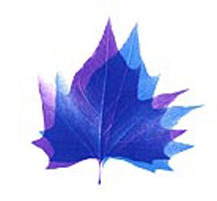
\includegraphics[width=0.15\textwidth]{Brighton-University-logo.png}\par
	{\scshape\LARGE University of Brighton\par}
	\vspace{1cm}
	{\scshape\Large Interim planning and Investigation report\par}
	\vspace{1.5cm}
	{\huge\bfseries Generation of Raspbian images\par}
	\vspace{2cm}
	{\Large\itshape Adam Pietrzycki\par}
	\vfill
	supervised by\par
	Dr.~Aidan \textsc{Delaney}
	\vfill

% Bottom of the page
	{\large \today\par}
\end{titlepage}

\begin{abstract}

\end{abstract}

\pagebreak
\tableofcontents
\pagebreak

\chapter{Introduction}
\section{Test}
This is a google \cite{google} bibliography test.
\section{Test 2}
Test 2
\subsection{Test 2a}
Test 2a

\chapter{Background Research}

\chapter{Design}

\begin{thebibliography}{9}
\bibitem{google} 
GoogleTest:
\\\url{https://google.com}
\end{thebibliography}

\end{document}